\chapter[Set-Membership Identification: intro, Equation-Error]{Set-Membership Identification: an introduction, Equation-Error noise structure}

The objective of this chapter is to introduce an approach for the parameter estimation which requires to do less strong assumption on the noise affecting the experimentally collected data. After a brief introduction with the crucial ingredients, we will go on with some instructive examples which will bring us to the complete formulation of the \textbf{Set-Membership System Identification procedure}.

\section{Ingredients for Set-Membership System Identification}
As usual in order to perform correctly the procedure of System Identification we need some crucial ingredients:
\begin{itemize}
    \itemsep-0.2em
    \item[\ding{182}] \textbf{\textsf{A-priori assumption on the system:}}
    \begin{enumerate}
        \item[\ding{51}] We use the general \textbf{regression form} 
        \begin{equation} 
            y(k)=f(y(k-1), y(k-2),  ..., y(k-n), u(k-1), ..., u(k-m), \theta)
        \end{equation}
        \item[\ding{51}] The \textbf{class of function} $\mathcal{F}$ and the order of the system $n$;     
    \end{enumerate}
   
    \item[\ding{184}] \textbf{\textsf{A-priori information of the noise}} and in particular:
    \begin{enumerate}  
        \itemsep-0.2em
        \item[\ding{51}] \textbf{Noise structure}: is referred to the way the uncertainty enters  into the problem.
        \item[\ding{51}] \textbf{Characteristic of the signal}, it is remarkable that here we assume something different and weaker. We will assume that the noise sequence/sequences (depending on the noise structure) belongs to a certain bounded set $\mathcal{B}$.
    \end{enumerate}
\end{itemize}

\section{Set-Membership Identification of LTI system with EE noise structure}
In this paragraph we will show what is obtained in term of parameter estimation, when we have that the a-priori information on the noise are the following:
\begin{itemize}
    \itemsep-0.3em
    \item[\ding{51}] The uncertainty enter in the problem as an additive term which we call $e(k)$ (the same of the first assumption of the theorem), that is:
    \begin{align*}
        y(k) = &-\theta_1{y(k-1)}-\theta_2{y(k-2)}-...-\theta_n{y(k-n)}\\
        &+\theta_{n+1}u(k)+\theta_{n+2}u(k-1)+...+\theta_{n+m+1}u(k-m) + \underbrace{e(k)}_{\textsf{EQUATION ERROR}}
    \end{align*}
    \item[\ding{51}] We suppose on the sequence characterizing the error is \textbf{bounded} (this is the crucial difference with respect to what requires the \textit{consistency theorem}), that is:
    \begin{equation}\label{eq:boundedness}
        e(k)\in\mathcal{B}_e \iff \vert e(k) \vert \le \Delta_e, \ k=1, ..., H
    \end{equation}
\end{itemize}
\subsection{Feasible Parameter Set $\mathcal{D}_\theta$}

\begin{quotation}
    \noindent
    \textsf{In this paragraph by using some examples, we will define the \textit{feasible parameter set} and its fundamental properties, in particular, it is useful to derive a \textbf{mathematical formulation of such a set} in order to explore its \textit{usefulness} and \textit{boundedness}}
\end{quotation}

\noindent
The set of solutions for the identification problem is implicitly described on what is called the \textbf{Feasible Parameter Set (FPS)}, we will indicate it with $\mathcal{D}_\theta$.

\begin{definition}[\textsf{\textbf{FEASIBLE PARAMETER SET}}] \textit{The \textbf{Feasible Parameter Set} $\mathcal{D}_\theta$ is the set of all the values of the parameter $\theta=[\theta_1 ... \theta_n]^T$ which are consistent (coherent) with all the available a-priori information (system and noise) and all the collected data (a-posteriori information).}
\end{definition}


\noindent
In order to better understand the meaning of $\mathcal{D}_\theta$ let us assume we are collecting data in the OE setup, and we know that $\vert \eta(k) \vert \le \Delta_\eta$. The input sequence, then, is perfectly known while the output is corrupted by the noise $\eta(k)$.

\begin{figure}[h]
    \centering
    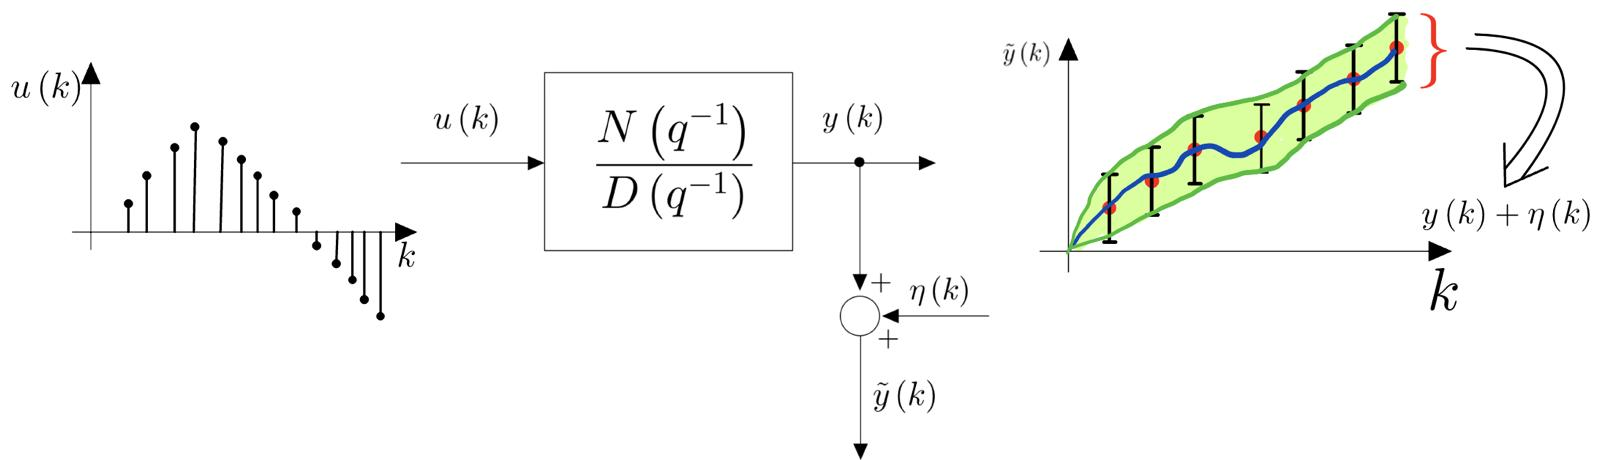
\includegraphics[scale=0.32]{img/oe_example.jpeg}
    \caption{OE set-up experiment}
\end{figure}

\noindent
The question is: \textsf{Is the SM approach providing us a pointwise estimate for the parameter $\theta$?} We will show more or less formally in the following that the answer is NO, but we can track an intuitive reasoning which will bring us to the same conclusion. \\
For this aim, given the sequence $u(k)$, we collect an output $\tilde{y}(k), \ k=0, 1, ...$. Moreover, let us suppose that for such collected data the obtained model is giving us some parameter $\theta$ such that the I/O mapping is the one indicated with the {\color{blue} blue} line. Now, since the output measurements are affected by noise, all of the samples between $[\tilde{y}(k)-\eta(k), \tilde{y}(k)+\eta(k)]$\footnote{
    See the black vertical bars
} is providing us an information which is coherent with the a-priori assumption on the noise itself. Besides, another couple of parameter $\theta_1, \theta_2$ derived from such samples, can be also the result of our identification problem. From the reasoning we have just presented we can intuitively understand that:
\begin{quotation} 
    \noindent
    \textsf{probably the parameter $\theta_i$ are provided with an \textbf{uncertainty interval} since also the experimental data are provided with uncertainty.}
\end{quotation}

\subsection{Mathematical formulation of the FPS}
We know that the system is a \textbf{second order}, \textbf{LTI one} (\textit{a-priori assumption on the system}), the uncertainty/noise enters the identification problem as additive term $e(k)$ (equation error) and it is \textbf{bounded} (that is $\vert e(k)\vert \le \Delta_e, \ k=0,1, ..., H$) (\textit{a-priori assumption on the noise}), after having collected the data $\tilde{y}(k)$, after having stimulated the system to be identified with a sequence $\tilde{u}(k)$ (\textit{a-posteriori information})\footnote{
    An EIV(Errors-in-variables) set-up is assumed, then, in order to be more precise the input is given by a subsystem, this is the reason why we have to measure it.
}, we can define the \textsf{Feasible Parameter Set} as follows:

\begin{equation} \label{eq:FPS_2nd}
    \begin{aligned}
        \mathcal{D}_\theta=&\{\theta\in\mathbb{R}^p: \ 
                \tilde{y}(k)=-\theta_1\tilde{y}(k-1)
                -\theta_2\tilde{y}(k-2)+\\
                &+\theta_3\tilde{u}(k)
                +\theta_4\tilde{u}(k-1)
                +\theta_5\tilde{u}(k-2)+e(k), \quad k=3,...,H\\
                &  \vert e(k) \vert \le \Delta_e, \quad k=1,...,H
        \}
    \end{aligned}
\end{equation}
The set (\ref{eq:FPS_2nd}) is made up of both inequality and equality constraints, moreover it appears clear that it is a \textit{subset of $\mathbb{R}^p$} with $p$ the number of parameters. There is a problem: the set $\mathcal{D}_\theta$ is defined using some inequality constraints on the noise samples $e(k)$ which are not part of the parameter space. In the following a way to eliminate such a dependence is shown, without adding any approximation or conservativeness.

\begin{equation*} 
    \begin{aligned}
        \mathcal{D}_\theta=&\{\theta\in\mathbb{R}^p: \ 
                \tilde{y}(k)+\theta_1\tilde{y}(k-1)
                +\theta_2\tilde{y}(k-2)+\\
                &-\theta_3\tilde{u}(k)
                -\theta_4\tilde{u}(k-1)
                -\theta_5\tilde{u}(k-2)=e(k), \quad k=3,...,H\\
                &  \vert e(k) \vert \le \Delta_e, \quad k=1,...,H
        \}= \\
        &\{\theta\in\mathbb{R}^p: \ 
                \vert \tilde{y}(k)+\theta_1\tilde{y}(k-1)
                +\theta_2\tilde{y}(k-2)+\\
                &-\theta_3\tilde{u}(k)
                -\theta_4\tilde{u}(k-1)
                -\theta_5\tilde{u}(k-2) \vert \le \Delta_e, \quad k=3,...,H
        \}
    \end{aligned}
\end{equation*}
In this way, we have obtained an implicit description of the \textbf{set of all the feasible solution of our identification problem} in term of a \textit{set of inequality contraints only involving $\theta$}.\\


\begin{multicols}{2}
    \noindent
    A graphical representation of such a set in a 2-dimensional parameter space is shown in the figure on the side. Here the objective is to analyze two main features of the Feasible Parameter Set by formulating the following two questions:  
    \normalsize{
    \begin{itemize}
        \itemsep-0.2em
        \item[(Q1)] \textsf{\textbf{\color{red}Boundedness}} Is this set a bounded one? Under which conditions?
        \item[(Q2)] \textsf{\textbf{\color{red}Usefulness}} What is the relation between $\mathcal{D}_\theta$ and $\theta_{\text{true}}$?
    \end{itemize}}
    \newcolumn
    \begin{center}
        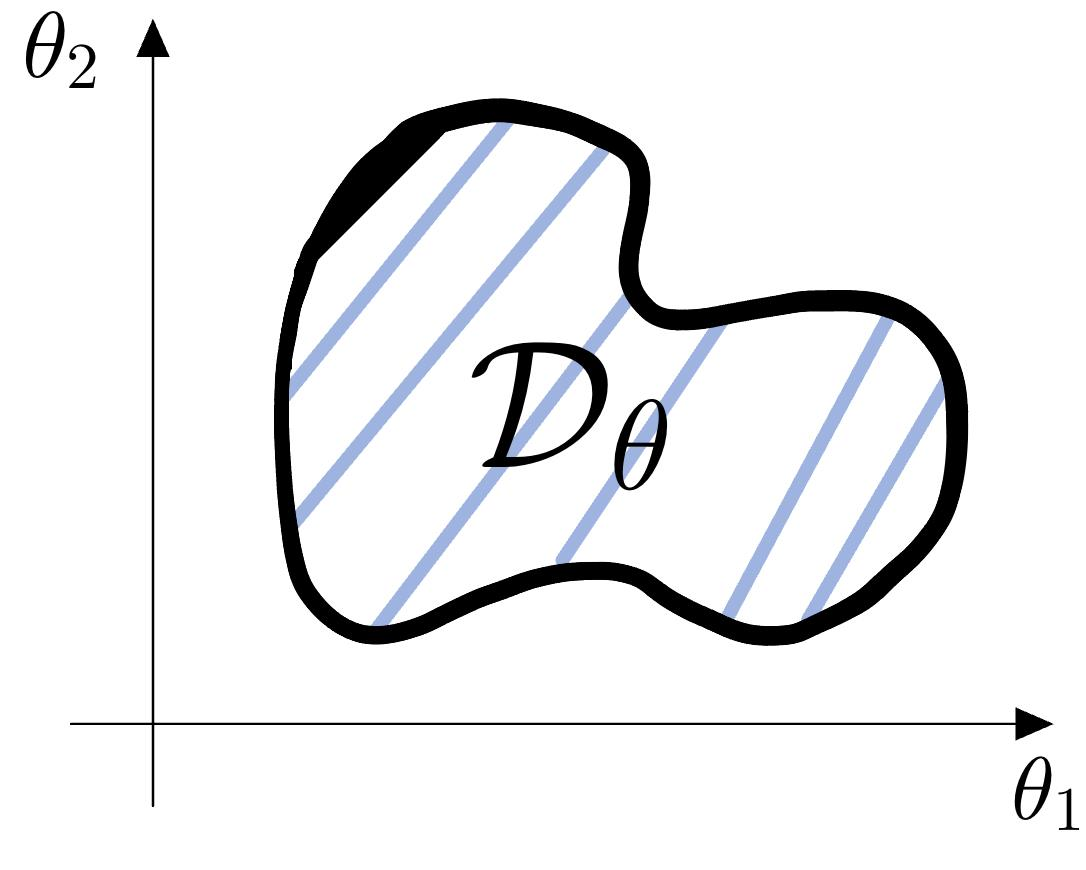
\includegraphics[scale=0.18]{img/FPS_1.jpeg}
    \end{center}
\end{multicols}
\subsubsection{Main features of $\mathcal{D}_\theta$}


\noindent
\textsf{\underline{Question Q1}} The boundedness of $\mathcal{D}_\theta$ depends on the way we collect the data (in general) ($\Rightarrow$ this concept has to be better specified in the next slides). \textit{For the moment let us assume that such a set is bounded}.\\

\noindent
\textsf{\underline{Question Q2}} Assuming that the a-priori assumptions on the system and on the noise are correct, then $\theta_{\text{true}}$ is guaranteed to belong to $\mathcal{D}_\theta$ (this is very important for further theory development).\\

\noindent
Once that we have obtained an implicit description of $\mathcal{D}_\theta$, \textit{how can we extract a useful model from it,either for simulating the system or designing a feedback controller for such a system?} Before saying it, we have to  distinguish \textit{two different classes} of SM estimation algotrithms: 
\begin{itemize}
    \itemsep-0.2em
    \item[(E1)] \textsf{\textbf{\color{red} Set-valued estimators}}, defined as estimation algorithms which provides a (possibly) conservative estimate of $\mathcal{D}_\theta$ in a \textbf{simplified geometrical form} that can be easily used to simulate or control the system; 
    \item[(E2)] \textsf{\textbf{\color{red} Pointwise Estimators}}, defined as estimation algorithms that provides a single value of $\theta$ which is an optimal estimate of $\theta_{\text{true}}$ in some sense.
\end{itemize}
Here, among all the possible estimator in the class (E1), we consider the algorithm which is providing the \textbf{minimum volume box outerbounding $\mathcal{D}_\theta$}. Such an estimator is implicitly providing what we will call \textbf{Parameter uncertainty Intervals (PUIs)}. 

\begin{multicols}{2}
    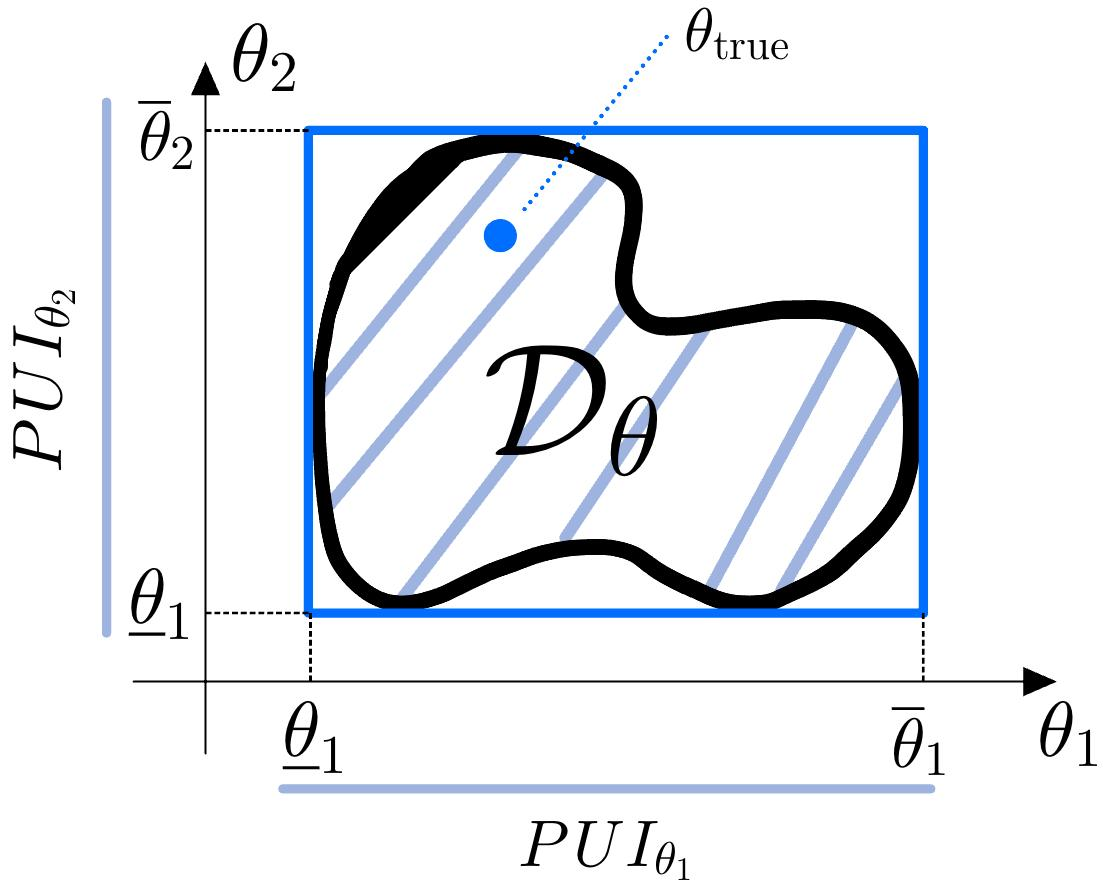
\includegraphics[scale=0.2]{img/PUI_1.jpeg}
    The PUI are defined as follows:
    \newcolumn
    \begin{equation}
        PUI_{\theta_j} = [\underline{\theta}_j,
        \overline{\theta}_j]
    \end{equation}
    where the extrema of the interval are:
    \begin{align}
        &\underline{\theta}_j \doteq \min_{\theta\in\mathcal{D}_\theta} {\theta_j}\\
        &\overline{\theta}_j \doteq \max_{\theta\in\mathcal{D}_\theta} {\theta_j} = \min_{\theta\in\mathcal{D}_\theta}{-\theta_j}
    \end{align}
    It is remarkable that each $PUI$ is providing the \textbf{minimum uncertainty interval} for each parameter $\theta_j$. In the figure are shown the $PUI$ for the feasible parameter set presented before.
\end{multicols}
\noindent 
Note the that, in the case of $\mathcal{D}_\theta \subseteq \mathbb{R}^2$ the minimum volume containing $\mathcal{D}_\theta$ is a rectangular shape whose sides are the parameter uncertainty intervals associated to $\theta_1$ and $\theta_2$.

\subsubsection{\color{orange}Usefulness of the PUIs}
Suppose you have for the following model, the corrensponding PUIs:
\begin{equation*}
    G(z)=\frac{\theta_2}{z+\theta_1} \quad
    \theta_2 \in [\underline{\theta}_2, \ \overline{\theta}_2] = PUI_{\theta_2}, \quad
    \theta_1 \in [\underline{\theta}_1, \ \overline{\theta}_1] = PUI_{\theta_1}
\end{equation*}
Moreover, you assume you want to derive a Lead/Lag controller for such a system. It is well known that the main idea behind this approach is having a representation of the loop function $L(s)$, and adding a certain number of dynamic networks in order to change the shape of $L(s)$ itself, in order to obtain a certain $\omega_{c, des}$ In this framework, we have not a single loop function but a cloud of them, from which we can retrieve a bound of  some type in order to derive a controller in the \textbf{limit cases}.

\begin{figure}[h]
    \centering
    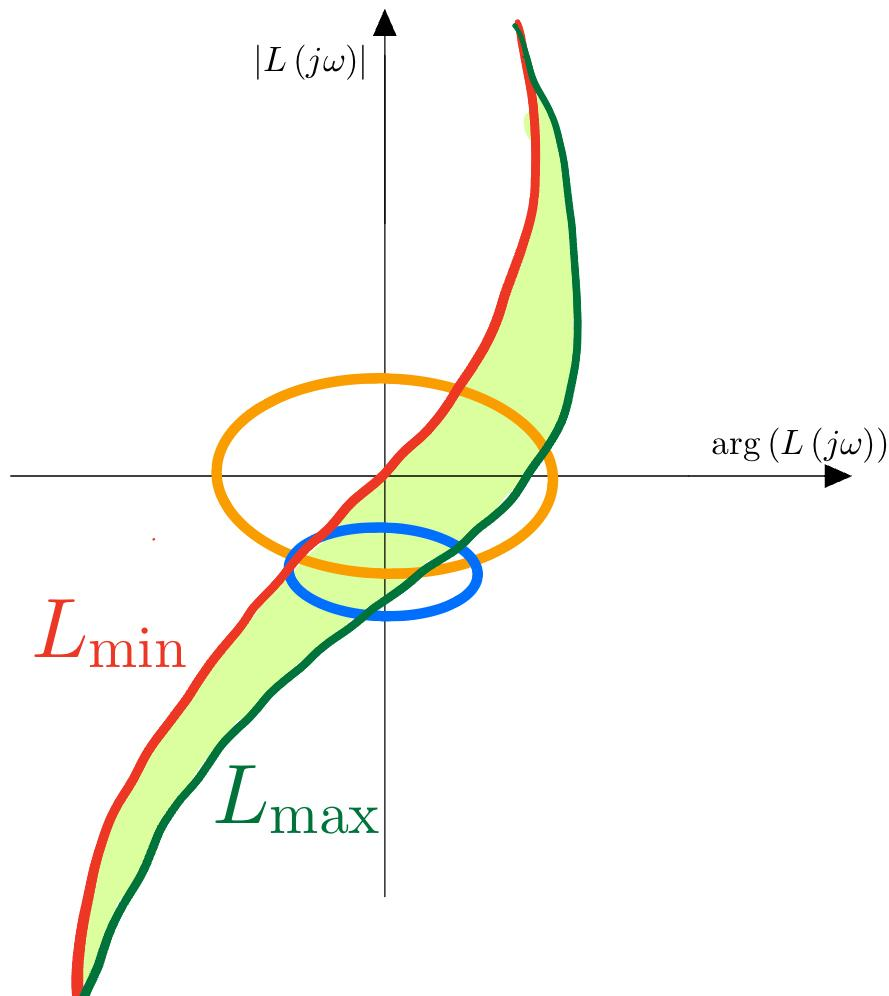
\includegraphics[scale=0.2]{img/Nichols.jpeg}
    \caption{Nichols plot of the loop function}
\end{figure}
At this aim, the following figure for example shows the \textit{frequency response} on the Nichols' Plot of the loop function. According to the choice of the parameters one can obtain a different plot in the range of curves delimited by $[L_{min}, L_{max}]$.

\subsection{Geometric shape of the Feasible Parameter Set}
In the case we have a linear time-invariant system where the uncertainty can be described by means of an unknown but bounded \textit{equation error} $e(k)$, we can obtain a particular shape of the FPS which makes the problem particularly 'simple' to solve. \\
For sake of simplicity, the description of such a property by using a first order system ($n=1$) is done. At this aim, we know that the transfer function has the shape:
\begin{equation}
    G(z)=\frac{\theta_2{z}}{z+\theta_1} \longrightarrow
    G({q^{-1}}) = \frac{\theta_2}{1+\theta_1{q^{-1}}}=\frac{y(k)}{u(k)}
\end{equation}
From which you can find that the regression form is:
\begin{equation}
    y(k)+\theta_1{y(k-1)}=\theta_2{u(k)} \iff 
    y(k) = -\theta_1{y(k-1)}+\theta_2{u(k)}
\end{equation}
This result has been issued by using the \textbf{a-priori information on the system}: LTI and $n=2$. On the other hand, we know that the noise enters the equation as an \textit{unknown but bounded} equation error $e(k)$, that is
\begin{equation*}
    \vert e(k) \vert \le \Delta_e   \quad k=1,..., N
\end{equation*}
Finally, the \textbf{a-posteriori information} are the experimentally collected data, which both are corrupted by measurement noise. 
\begin{equation*}
    \tilde{u}(k)=u(k)+\xi(k), \quad 
    \tilde{y}(k)=y(k)+\eta(k) \quad \forall k=1, ..., N
\end{equation*}
Putting all together, we can find the implicit mathematical formulation of the FPS as follows:

\begin{equation}
    \begin{aligned}
        \mathcal{D}_\theta = &\{
            \theta\in\mathbb{R}^2: \ 
            \tilde{y}(k)=-\theta_1\tilde{y}(k-1)+\theta_2{\tilde{u}(k)} + e(k), \quad k=2, ..., N, \\
            & \vert e(k) \vert \le \Delta_e   \quad k=1,..., N
        \}=\\
        &=\{\theta\in\mathbb{R}^2: \
            \vert
            \tilde{y}(k)+\theta_1\tilde{y}(k-1)-\theta_2{\tilde{u}(k)}
            \vert  \le \Delta_e, \quad k=2,..., N
        \}=\\
        &=\{ \theta\in\mathbb{R}^2: \ -\Delta_e \le 
            \tilde{y}(k)+\theta_1\tilde{y}(k-1)-\theta_2{\tilde{u}(k)}
            \le \Delta_e, \quad k=2,...,N
        \}=\\
        &=\{\theta\in\mathbb{R}^2: \
            {\color{red}\theta_1\tilde{y}(k)-\theta_2\tilde{u}(k) \le \Delta_e-\tilde{y}(k)} \quad \textsf{(C1)} \\
            &\qquad \qquad \quad{\color{blue}-\theta_1\tilde{y}(k)+\theta_2\tilde{u}(k) \le \Delta_e+\tilde{y}(k)} \quad \textsf{(C2)}, \quad k=2, ..., N
        \}
    \end{aligned}
\end{equation}
\noindent
For each $k$, from $\mathcal{D}_\theta$ we obtain a couple of straight lines. Let us represent them by computing the constraints $\textsf{(C1)}$ and $\textsf{(C2)}$ for $k=2,3$

\subsubsection{Constraints for \color{red} $k=2$}
\begin{align}
    \tag{\color{red}\textsf{C1}}
    &\begin{aligned}\label{eq:c1_1}
        &\tilde{y}(2)+\theta_1{\tilde{y}(1)}-\theta_2\tilde{u}(2) \le \Delta_e \\
        &\theta_2 \ge \frac{\tilde{y}(1)}{\tilde{u}(2)}\theta_1 + \frac{\tilde{y}(2)-\Delta_e}{\tilde{u}(2)}
    \end{aligned}\\
    \tag{\color{blue}\textsf{C2}}
    &\begin{aligned}\label{eq:c1_1}
        &\tilde{y}(2)+\theta_1{\tilde{y}(1)}+\theta_2\tilde{u}(2) \le -\Delta_e \\
        &\theta_2 \le \frac{\tilde{y}(1)}{\tilde{u}(2)}\theta_1 + \frac{\tilde{y}(2)+\Delta_e}{\tilde{u}(2)}
    \end{aligned}
\end{align}
We can note that such lines have the \textbf{same angular coefficient} but different \textbf{intercept}. Roughly speaking they are parallel straight lines, that in form of inequalities define some \textit{halfplanes}. Since in the FPS the constraints must be satisfied \textbf{for each $k$}, we take the intersection of such constraints. In the specific case they result in a \textbf{strip}. Such a set is unbounded, this is related to the fact we used a single constraints against two degree of freedom (that is 2 parameters). 

\begin{figure}[h]
    \centering
    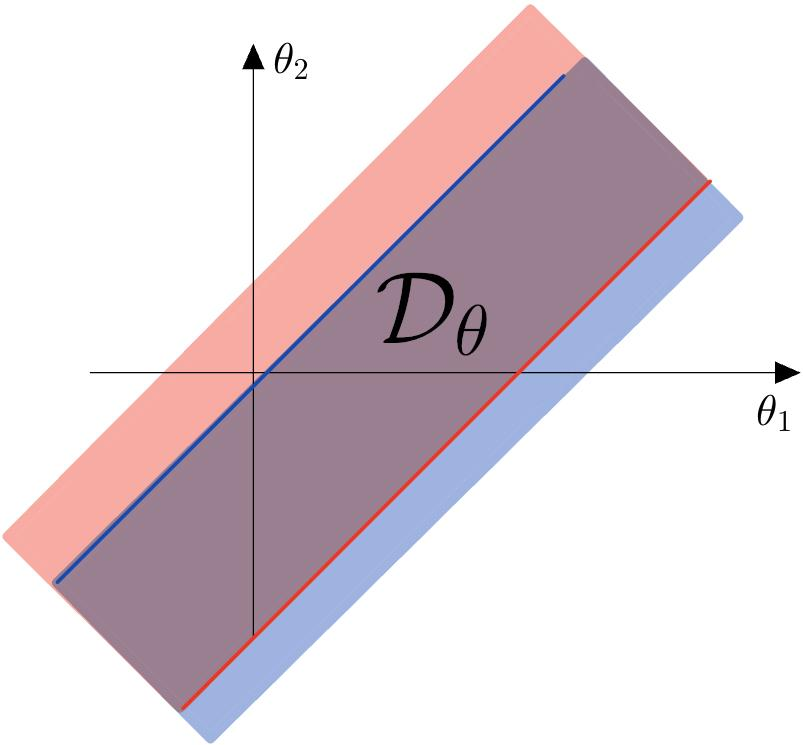
\includegraphics[scale=0.22]{img/strip.jpeg}
    \caption{$\mathcal{D}_\theta$ resulting from a single equation}
\end{figure}
\noindent
A possible representation is given in the figure above. Now, in order to obtain a bounded set we must collect $k=3$ data while using at least 2 equations resulting in 2 pairs of constraints $\textsf{C1-C2}$.
\subsubsection{Constraints for \color{red} $k=3$}
Following the same reasoning we obtain:
\begin{align}
    \tag{\color{red}\textsf{C1}}
    &\begin{aligned}\label{eq:c1_1}
        &\tilde{y}(3)+\theta_1{\tilde{y}(2)}-\theta_2\tilde{u}(3) \le \Delta_e \\
        &\theta_2 \ge \frac{\tilde{y}(2)}{\tilde{u}(3)}\theta_1 + \frac{\tilde{y}(3)-\Delta_e}{\tilde{u}(3)}
    \end{aligned}\\
    \tag{\color{blue}\textsf{C2}}
    &\begin{aligned}\label{eq:c1_1}
        &\tilde{y}(3)+\theta_1{\tilde{y}(2)}+\theta_2\tilde{u}(3) \le -\Delta_e \\
        &\theta_2 \le \frac{\tilde{y}(2)}{\tilde{u}(3)}\theta_1 + \frac{\tilde{y}(3)+\Delta_e}{\tilde{u}(3)}
    \end{aligned}
\end{align}

\noindent
Combining the two halfplanes with the ones obtained before, we obtain that \textbf{intersection is a convex set}, and in particular is a \textbf{polytope}. Note that the angular coefficient for the couple of lines derived putting $k=3$, clearly is different than the one we have obtained for $k=2$.

\begin{figure}[h]
    \centering
    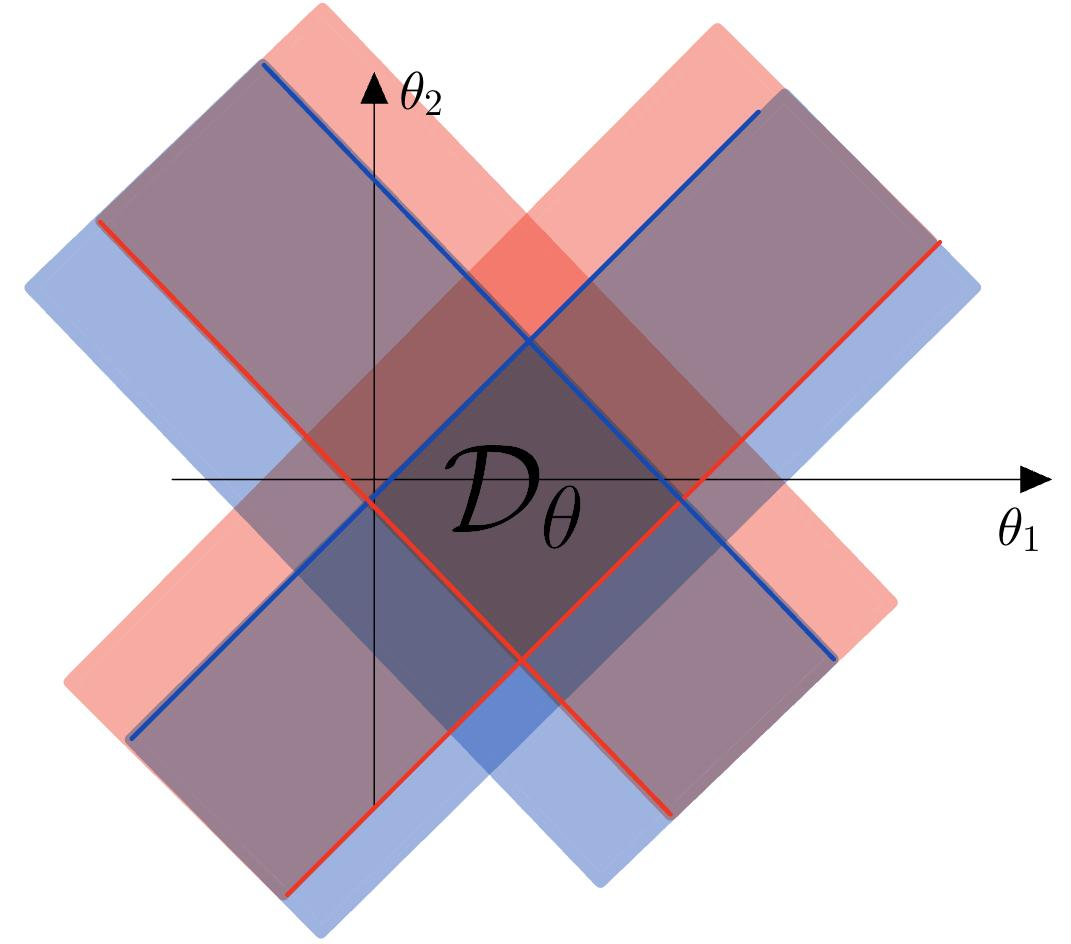
\includegraphics[scale=0.2]{img/polytope1.jpeg}
    \caption{$\mathcal{D}_\theta$ resulting from a pair of equations}
\end{figure}

{\color{blue}
\noindent
Let us remind that the FPS for sure contains $\theta_{true}$
if and only if all the a-priori assumptions are correct, otherwise the FPS will be \textbf{empty}!}\\
It is remarkable, that this was a case in which by inspection you can read the $PUI$, however we need to generalize. In particular the problem of finding a $PUI$ in the hypotesis of LTI systems with equation error noise structure can be recasted in the solution of \textbf{two standard Linear Programming (LP) problems}: minimization of a linear (convex) objective under constraints representing a polytope.\footnote{
    \noindent
    A \textbf{Linear Programming (LP) problem} is a convex optimization problem of the form
    \begin{equation*}
        \min_{x\in\mathbb{R}^n} {c^T{x}} \quad \text{subject to} \ Ax \le b
    \end{equation*}
    This takes into account all the situations when the problem can be \textit{exactly written} as the minimization of a \textbf{linear function} of the optimization variable subject to \textbf{a set of linear inequalities and/or equalities constraints}.
}

\section{PUIs computation by mean of LP problems solution} 
We know that for a certain parameter $\theta_j$, $j=1,...,p$,  the related interval is $PUI=[\underline{\theta}_j, \overline{\theta}_j]$. Under assumption of having a LTI system with Unknown But Bounded error.
\begin{align}
    \label{eq:th_under}
    &\underline{\theta}_j \doteq \min_{\theta\in\mathcal{D}_\theta} \theta_j= \min_{\theta\in\mathbb{R}^n} \theta_j 
    \qquad \qquad \qquad  \text{s.t.} \begin{cases}
        \tilde{y}(k)+... \le \Delta_e\\
        \tilde{y}(k)+... \le -\Delta_e
    \end{cases} \ k=n+1, ..., N\\
    \label{eq:th_over}
    &\overline{\theta}_j \doteq \max_{\mathcal{D}_\theta} {\theta_j} = \max_{\theta\in\mathbb{R}^n} {\theta_j}=\min_{\theta\in\mathbb{R}^n} {-\theta_j} 
    \quad  \text{s.t.} \begin{cases}
        \tilde{y}(k)+... \le \Delta_e\\
        \tilde{y}(k)+... \le -\Delta_e
    \end{cases} \ k=n+1, ..., N
\end{align}

\noindent
Note that both the problems (\ref{eq:th_under}) and (\ref{eq:th_over}) can be rewritten in the form of an LP problem by suitably choosing $c$ and by arranging the set of constraints in suitable matrices $A$ and $b$. For example when we want to compute the PUI for the $\theta_1$ parameter for a first order system, the direction $c$ will be $c=[1 \quad 0]^T$, then for $\theta_2$, $c=[0 \quad 1]^T$. In \texttt{MATLAB} once you have formulated the problem in the LP form, you can use the command \texttt{[th, opt\_val]=linprog(c,A,b)}, in which \texttt{th} is the optimal solution, while \texttt{opt\_val} is the optimization variable.\\
In conclusion, we have understood that the problem of finding the PUIs for $p$ parameters in the described setting, is leading to the solution of $2p$ LP problems, whose solutions are \textbf{global ones}, the problem in this case can be exactly solved without adding any conservativeness!\\

\noindent
The most critical issue of using such an approach is that, despite any type of experimental set-up can be recasted into a model having an equation error noise structure, I rarely am able to retrieve a bound $\Delta_e$. \\
{\color{blue}
More in particular, this approach can be applied all the times you have that the model is linearly parametrized, that is \textit{the parameters appears linearly in the equation}, since from the regression form you have samples from the input and output which can be for sure non linear ones! 
}


\section{Final remarks}
In this section we have introduced the \textit{Set-Membership approach} for the model parameters estimation. Next, we have analysed the main ingredients, and introducing the concept of \textbf{Feasible parameter set} we have understood that such an approach leads with itself a robust way for describing the parameters, embedding the uncertainty which comes from the data collection. This has been carried out by properly defining the \textit{Parameter Uncertainty Interval}. \\

In the last part we have applied all of the features of the described approach starting from the simplest case in which the model to be identified was LTI and the noise samples unknonwn but bounded. By suitably arranging the mathematical constraints derived by putting together all the a-priori and a-posteriori information, we have recasted the problem of finding the PUIs in the solution of a couple of LP problems which leads to a global minima. Finally, analyzing the problem of SM Identification in this way was mainly of theoretical and conceptual interest since we have seen that retrieving a bound $\Delta_e$ on the error is practically impossible. Other approaches embedding a complete description of the noise samples are needed.

\section*{References}

\begin{itemize}
    \itemsep-0.3em
    \item[\Large{\ding{45}}]  \Citeauthor{milanese2013bounding}, \textit{\citetitle{milanese2013bounding}}, \citedate{milanese2013bounding}
    \item[\Large{\ding{45}}]  \Citeauthor{milanese1982estimation}, \textit{\citetitle{milanese1982estimation}}, \citedate{milanese1982estimation}
\end{itemize}